\documentclass[aspectratio=169]{ctexbeamer} %[t]:顶端对齐
\usepackage{array}
\makeatletter
\def\input@path{{../../styles}}  % 
\makeatother
\usepackage{ubeamer}
\uBigPaper
\uSetBigFont

\date{\today}

\title{集合与逻辑用语}

\begin{document}

\begin{frame}
\titlepage
\end{frame}

\begin{frame}
\frametitle{目录}
\tableofcontents
\end{frame}

\section{集合的概念}

\begin{frame}
\frametitle{集合的概念}
\begin{itemize}
\item \textbf{集合的定义}:一般地,我们把研究对象统称为\alert{元素}(element),把一些元素组成的总体叫做\alert{集合}(set)(简称集)。
\item \textbf{特征}:
  \begin{itemize}
  \item \textbf{确定性}:给定的集合,它的元素必须是确定的。也就是说,给定一个集合,那么一个元素在或不在这个集合中,就确定了。
  \item \textbf{互异性}:一个给定集合中的元素是互不相同的。也就是说,集合中的元素是不重复出现的。
  \item \textbf{无序性}:集合中的元素没有顺序。
  \end{itemize}
\end{itemize}
\end{frame}

\section{集合的表示方法}

\begin{frame}
\frametitle{集合的表示方法}
\begin{itemize}
\item \textbf{列举法}:把集合的元素一一列举出来,并用花括号“\{\}”括起来。例如,方程 \(x^2 - 1 = 0\) 的所有实根组成的集合表示为 \(\{-1, 1\}\)。\\
\item \textbf{描述法}:用集合所含元素的共同特征表示集合。形式为:\(\{x | x\) 具有的性质\}。例如,不等式 \(x - 3 > 2\) 的解集可表示为 \(\{x | x > 5\}\)。
\end{itemize}
\end{frame}

\section{元素与集合的关系}
\begin{frame}
\frametitle{元素与集合的关系}
通常,用大写拉丁字母\(A, B, C, \cdots \)表示集合,用小写拉丁字母\(a, b, c, \cdots \)表示集合中的元素。\\
\begin{itemize}
\item \textbf{属于}:若元素 \(a\) 是集合 \(A\) 的元素,则称 \(a\) \alert{属于}(belong to) \(A\),记为 \(a \in A\)。\\
\item \textbf{不属于}:若元素 \(a\) 不是集合 \(A\) 的元素,则称 \(a\) \alert{不属于} \(A\),记为 \(a \notin A\)。\\
\item \textbf{举例}:集合 \(A = \{1, 2, 3\}\),则 \(1 \in A\),\(4 \notin A\)。
\end{itemize}
\end{frame}

%常用数集
\begin{frame}
\frametitle{常用数集}
\begin{table}[h]
\centering
\begin{tabular}{|m{5cm}|m{5cm}|m{20cm}|}
\hline
\textbf{数集名称} & \textbf{记法} & \textbf{定义} \\ \hline
自然数集 & $\mathbb{N}$ & 表示非负整数的集合,即 $\mathbb{N} = \{0, 1, 2, 3, \ldots\}$。在某些数学文献或教材中,自然数集也可能从1开始,即 $\mathbb{N} = \{1, 2, 3, \ldots\}$,但通常以包含0为主。 \\ \hline
正整数集 & $\mathbb{N}^*$ 或 $\mathbb{N}_+$ & 表示正整数的集合,即 $\mathbb{N}^* = \{1, 2, 3, \ldots\}$。 \\ \hline
整数集 & $\mathbb{Z}$ & 表示所有整数(正整数、零和负整数)的集合,即 $\mathbb{Z} = \{\ldots, -2, -1, 0, 1, 2, \ldots\}$。 \\ \hline
有理数集 & $\mathbb{Q}$ & 表示可以表示为两个整数之比(分母不能为零)的数的集合,即 $\mathbb{Q} = \left\{ \dfrac{a}{b} \mid a \in \mathbb{Z}, b \in \mathbb{Z}, b \neq 0 \right\}$。 \\ \hline
实数集 & $\mathbb{R}$ & 表示包括有理数和无理数在内的所有实数的集合。实数集可以用来表示连续的量,包括整数、分数、无限不循环小数等。 \\ \hline
\end{tabular}
\end{table}

\end{frame}

%集合间的基本关系
\section{集合间的基本关系}
\begin{frame}
\frametitle{集合间的基本关系}
\begin{itemize}
\item \alert{\textbf{子集}}:对于集合 \(A\) 和 \(B\),若 \(A\) 中任意元素都是 \(B\) 中的元素,则称 \(A\) 是 \(B\) 的子集,记为 \(A \subseteq B\)。例如,\(A = \{1, 2\}\),\(B = \{1, 2, 3\}\),则 \(A \subseteq B\)。\\
\item \alert{\textbf{真子集}}:若 \(A\) 是 \(B\) 的子集,且 \(B\) 中至少有一个元素不属于 \(A\),则称 \(A\) 是 \(B\) 的真子集,记为 \(A \subsetneqq B\)或\(B \supsetneqq  A \),读作\(A\)真包含于\(B\),或\(B\)真包含\(A\)。
\item 例如,\(A = \{1\}\),\(B = \{1, 2\}\),则 \(A \subsetneqq B\),或\(B \supsetneqq  A \)。\\
\item \alert{\textbf{相等}}:若 \(A\) 是 \(B\) 的子集,且 \(B\) 也是 \(A\) 的子集,则 \(A\) 与 \(B\) 相等,记为 \(A = B\)。例如,\(A = \{1, 2\}\),\(B = \{2, 1\}\),则 \(A = B\)。
\end{itemize}
\end{frame}

\section{集合的基本运算}
\begin{frame}
\frametitle{集合的基本运算}
\begin{itemize}
\item \textbf{\alert{并集}}:由属于集合 \(A\) 或属于集合 \(B\) 的所有元素组成的集合,称为 \(A\) 与 \(B\) 的并集,记为 \(A \cup B\)。即 \(A \cup B = \{x | x \in A \text{ 或 } x \in B\}\)。例如,\(A = \{1, 2, 3\}\),\(B = \{3, 4, 5\}\),则 \(A \cup B = \{1, 2, 3, 4, 5\}\)。\\

\item \textbf{\alert{交集}}:由既属于集合 \(A\) 又属于集合 \(B\) 的所有元素组成的集合,称为 \(A\) 与 \(B\) 的交集,记为 \(A \cap B\)。即 \(A \cap B = \{x | x \in A \text{ 且 } x \in B\}\)。例如,\(A = \{1, 2, 3\}\),\(B = \{3, 4, 5\}\),则 \(A \cap B = \{3\}\)。\\

\item \textbf{\alert{补集}}:设 \(S\) 是一个集合,\(A\) 是 \(S\) 的子集,由 \(S\) 中不属于 \(A\) 的所有元素组成的集合称为 \(S\) 中子集 \(A\) 的补集,记为 \(\complement_S A\)。即 \(\complement_S A = \{x | x \in S \text{ 且 } x \notin A\}\)。例如,\(S = \{1, 2, 3, 4, 5\}\),\(A = \{1, 2\}\),则 \(\complement_S A = \{3, 4, 5\}\)。
\end{itemize}
\end{frame}

% Venn图(文氏图)
\begin{frame}
\frametitle{Venn图(文氏图)}
\begin{itemize}
\item Venn图(文氏图)是一种用于展示集合及其关系的直观图形工具。它通过封闭曲线(通常是圆形)来表示集合,曲线内部的区域表示集合中的元素,外部则表示不属于该集合的元素。Venn图由英国逻辑学家约翰・维恩(John Venn)在19世纪末期提出,因此得名。
\item 单个集合的Venn图 :用一个简单的封闭曲线(通常是圆或椭圆)表示一个集合。例如,要表示集合A,可以画一个圆,并在圆内写下属于集合A的元素,圆外则表示不属于集合A的元素。
\item 多个集合的Venn图 :当有多个集合时,Venn图通过重叠的封闭曲线来展示它们之间的关系。如两个集合A和B的Venn图,画两个重叠的圆,重叠部分表示同时属于A和B的元素(即$A \cap B$),不重叠的部分分别表示只属于A或只属于B的元素。
\end{itemize}

\begin{figure}[h]
\centering
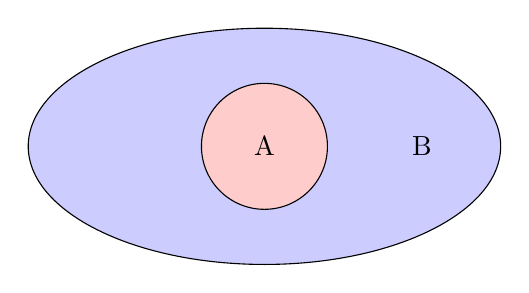
\begin{tikzpicture}
% 绘制集合B(椭圆)
\draw[fill=blue!20] (3,0) ellipse (3cm and 1.5cm);
% 绘制集合A(圆形),使其完全包含在B内
\draw[fill=red!20] (3,0) circle (0.8cm);
% 添加标签
\node at (3,0) {A};
\node at (5, 0) {B}; % 将B的标注放在椭圆内
\end{tikzpicture}
\label{venn:subset_ellipse}
\end{figure}

\end{frame}

% 练习
\begin{frame}
\frametitle{练习}
\begin{enumerate}[label={\arabic*.}]
\item 写出集合\(\{a, b, c\}\)的所有子集。
\item 用适当的符号填空:\\
(1) $a \underline{\hspace{2em}} \{a, b, c\}$;\hspace{3cm} (2) $0 \underline{\hspace{2em}} \{ x | x^2 = 0 \}$;\\
(3) $\varnothing \underline{\hspace{2cm}} \{ x \in \mathbb{R} | x^2 + 1 = 0 \} $;\hspace{3cm} (4);$\{0, 1\} \underline{\hspace{2em}} \mathbb{N}$
\end{enumerate}
\end{frame}

\section{充分必要条件}
\begin{frame}
\frametitle{命题及其关系}
\begin{itemize}
\item \textbf{命题定义}:用语言、符号或式子表达的,可以判断真假的陈述句称为命题。
\item 判断为真的语句称为真命题,判断为假的语句称为假命题。
\item 若 \(p\),则 \(q\);或者:如果\(p\),那么\(q\)。其中,\(p\)称为命题的条件,\(q\)称为命题的结论。
\item \textbf{四种命题}:
  \begin{itemize}
  \item \textbf{原命题}:若 \(p\),则 \(q\);
  \item \textbf{逆命题}:若 \(q\),则 \(p\);
  \item \textbf{否命题}:若非 \(p\),则非 \(q\);
  \item \textbf{逆否命题}:若非 \(q\),则非 \(p\)。
  \end{itemize}
\end{itemize}
\end{frame}

\begin{frame}
\frametitle{充分条件、必要条件、充要条件}
\begin{enumerate}[label={\arabic*.}]
\item \textbf{充分条件、必要条件}:若 \(p\),则 \(q\);我们说,$p$可以推出$q$,记作$p \Rightarrow q$。并且说,$p$是$q$的\alert{充分条件}(sufficient condition),$q$是$p$的\alert{必要条件}(necessary condition)。\\

\item 如果“若 \(p\),则 \(q\)”为假命题,那么由条件$p$不能推出结论$q$,记作$p \nRightarrow q$。此时,我们就说,$p$不是$q$的\alert{充分条件},$q$不是$p$的\alert{必要条件}。\\

\item \textbf{充要条件}:如果“若 \(p\),则 \(q\)”和它的逆命题“若 \(q\),则 \(p\)”都是真命题,即既有$p \Rightarrow q$,又有$q \Rightarrow p$,就记作$p \iff q$。此时,$p$既是$q$的\alert{充分条件},有是$q$的\alert{必要条件},我们说$p$是$q$的\alert{充分必要条件},简称为\alert{充要条件}(necessary and sufficient condition)。

\end{enumerate}
\end{frame}\section{简单的逻辑联结词}
\begin{frame}
\frametitle{简单的逻辑联结词}
\begin{enumerate}[label={\arabic*.}]
\item \textbf{逻辑与(\(\land\))}:用联结词“且”把命题 \(p\) 和命题 \(q\) 联结起来,得到新命题 \(p \land q\)。当 \(p\)、\(q\) 均为真时,\(p \land q\) 为真;当 \(p\)、\(q\) 中有一个为假时,\(p \land q\) 为假。\\

\item \textbf{逻辑或(\(\lor\))}:用联结词“或”把命题 \(p\) 和命题 \(q\) 联结起来,得到新命题 \(p \lor q\)。当 \(p\)、\(q\) 中有一个为真时,\(p \lor q\) 为真;当 \(p\)、\(q\) 均为假时,\(p \lor q\) 为假。\\

\item \textbf{逻辑非(\(\neg\))}:对命题 \(p\) 全盘否定,得到新命题 \(\neg p\)。若 \(p\) 为真,则 \(\neg p\) 为假;若 \(p\) 为假,则 \(\neg p\) 为真。\\

\end{enumerate}
\end{frame}

\section{全称量词与存在量词}
\begin{frame}
\frametitle{全称量词与存在量词}
\begin{itemize}
\item \textbf{全称量词}:短语“对所有的”、“对任意一个”称为全称量词,用符号“\(\forall\)”表示。含有全称量词的命题称为全称命题。例如,对任意 \(x \in \mathbb{R}\),\(x > 1\),记作 \(\forall x \in \mathbb{R}\),\(x > 1\)。\\

\item \textbf{存在量词}:短语“存在一个”、“至少有一个”称为存在量词,用符号“\(\exists\)”表示。含有存在量词的命题称为特称命题(或存在性命题)。例如,存在 \(x \in \mathbb{R}\),\(x > 1\),记作 \(\exists x \in \mathbb{R}\),\(x > 1\)。
\end{itemize}
\end{frame}

\section{全称量词命题与存在量词命题的否定}
\begin{frame}
\frametitle{全称量词命题的否定与存在量词命题的否定}
\begin{itemize}
\item \textbf{全称量词命题}:  \(\forall x \in \mathbb{M}\),\(p(x)\)。\\

\item \textbf{它的否定命题}: \(\exists x \in \mathbb{M}\),\(\neg p(x) \)。 \\

\item \textbf{存在量词命题}:  \(\exists x \in \mathbb{M}\),\(p(x)\)。\\

\item \textbf{它的否定命题}: \(\forall x \in \mathbb{M}\),\(\neg p(x) \)。 \\
\item \alert{由此可见,全称量词名词的否定是存在量词命题;存在量词命题的否定是全称量词命题。}
\end{itemize}
\end{frame}

%总结
\section{总结}

\begin{frame}
\frametitle{总结}
本节课我们学习了集合的概念、表示方法、元素与集合的关系、集合间的基本关系、集合的基本运算,以及命题及其关系、简单的逻辑联结词、全称量词与存在量词等内容。这些知识是高中数学的基础,希望大家能够熟练掌握。
\end{frame}

\section{练习}

\begin{frame}
\frametitle{练习}
\begin{enumerate}[label={\arabic*.}]
\item 用列举法表示集合 \(A = \{x \in \mathbb{N} | 0 < x < 5\}\)。
\item 判断下列命题的真假:若 \(x > 0\),且 \(y > 0\),则 \(x + y > 0\)。
\item 写出命题“若 \(a > 0\),则 \(a^2 > 0\)”的逆命题、否命题和逆否命题,并判断它们的真假。
\end{enumerate}
\end{frame}

\section{例题}
\begin{frame}
\frametitle{例题}
\begin{block}{例题1}
给定集合 \(A = \{1, 2, 3, 4, 5\}\),判断以下元素是否属于集合 \(A\):\\
$A. \, 2.5 \quad B.\, 3 \quad C.\, 4 \quad D. \, 6$
\end{block}
\pause
集合 \(A\) 的元素为 1, 2, 3, 4, 5,因此:2.5 不属于集合 \(A\),3 属于集合 \(A\),4 属于集合 \(A\),6 不属于集合 \(A\)。\\
\( 2.5 \notin A, \quad 3 \in A, \quad 4 \in A, \quad 6 \notin A.\)
\end{frame}

\begin{frame}{例题 2:集合的基本运算}
给定集合 \(A = \{1, 2, 3\}\),集合 \(B = \{3, 4, 5\}\)。求以下集合:
\begin{itemize}
    \item 并集:\(A \cup B\)
    \item 交集:\(A \cap B\)
    \item 差集:\(A - B\)
    \item 差集:\(B - A\)
\end{itemize}
\pause
\textbf{解析:}
\begin{itemize}
    \item 并集 \(A \cup B\) 包含所有属于 \(A\) 或属于 \(B\) 的元素。因此,\(A \cup B = \{1, 2, 3, 4, 5\}\)。
    \item 交集 \(A \cap B\) 包含所有同时属于 \(A\) 和 \(B\) 的元素。因此,\(A \cap B = \{3\}\)。
    \item 差集 \(A - B\) 包含所有属于 \(A\) 但不属于 \(B\) 的元素。因此,\(A - B = \{1, 2\}\)。
    \item 差集 \(B - A\) 包含所有属于 \(B\) 但不属于 \(A\) 的元素。因此,\(B - A = \{4, 5\}\)。
\end{itemize}
\end{frame}

\begin{frame}{例题 3:判断命题的真假}
判断以下命题的真假:
\begin{itemize}
    \item 命题 \(p\):若 \(x > 0\) 且 \(y > 0\),则 \(x + y > 0\)。
    \item 命题 \(q\):若 \(x\) 是偶数,则 \(x^2\) 也是偶数。
\end{itemize}
\pause
\textbf{解析:}
\begin{itemize}
    \item 对于命题 \(p\),假设 \(x\) 和 \(y\) 都是正数,那么 \(x + y\) 的和也一定是正数。因此,命题 \(p\) 为真。
    \item 对于命题 \(q\),假设 \(x\) 是偶数,即 \(x = 2k\)(\(k\) 为整数),则 \(x^2 = (2k)^2 = 4k^2 = 2 \cdot (2k^2)\),显然 \(x^2\) 也是偶数。因此,命题 \(q\) 为真。
\end{itemize}
\end{frame}

\begin{frame}{例题 4:逻辑联结词的应用}
给定命题 \(p\):今天下雨;命题 \(q\):今天刮风。写出以下复合命题的符号表示,并判断其真假(假设今天既下雨又刮风):
\begin{itemize}
    \item \(p\) 且 \(q\)
    \item \(p\) 或 \(q\)
    \item 非 \(p\)
\end{itemize}
\pause
\textbf{解析:}
\begin{itemize}
    \item \(p\) 且 \(q\) 的符号表示为 \(p \land q\)。由于今天既下雨又刮风,因此 \(p\) 和 \(q\) 都为真,所以 \(p \land q\) 为真。
    \item \(p\) 或 \(q\) 的符号表示为 \(p \lor q\)。由于 \(p\) 和 \(q\) 都为真,因此 \(p \lor q\) 为真。
    \item 非 \(p\) 的符号表示为 \(\neg p\)。由于 \(p\) 为真,因此 \(\neg p\) 为假。
\end{itemize}
\end{frame}

\end{document}